\chapter*{Highlevel Architecture}

\begin{figure}[h]
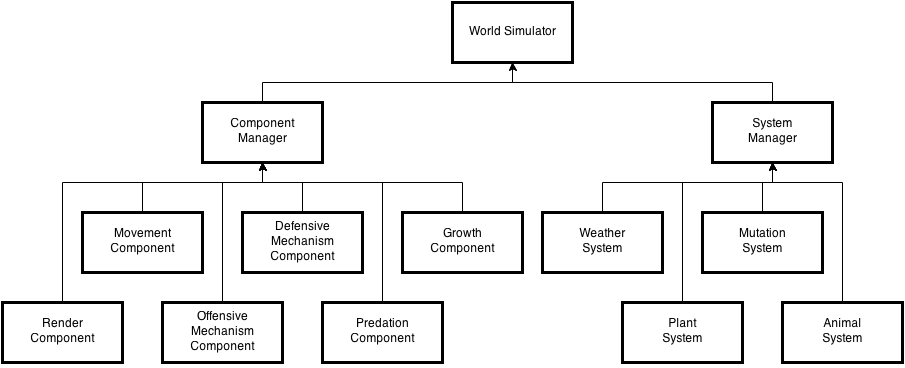
\includegraphics[width=\textwidth]{architecture.png}
\caption{High Level Architecture Diagram}
\label{fig:arch}
\end{figure}

Figure~\ref{fig:arch} shows a block level diagram of the GWS system and its various parts.

\begin{description}
\item[World Simulator] This is the host that will house the various Systems of the world to be simulated
\item[Component Manager] Manages the components that will make up entities (an entity is a representation of a single organism in the world).
\item[System Manager] Manages all the systems that will interact with the world. For example, the WeatherSystem will interact with the oxygen, water, and heat level in the world.
\end{description}

We will utilize object composition in a manner known as Entity-Component Architecture to model alien organisms (entities) in an alien environment (made up of various Systems). Each entity is made up of different Components in order to provide room for growth and mutation. For example, a kind of alien plant might not have Movement or Offensive components (this particular alien plant cannot move), but will definitely have Growth and Mating components. On the other hand, a different alien plant might be able to move and thus will have a Movement component.

Figure~\ref{fig:comp} describes a Component system that is similar to what we will implement in our project.

\begin{figure}[h]
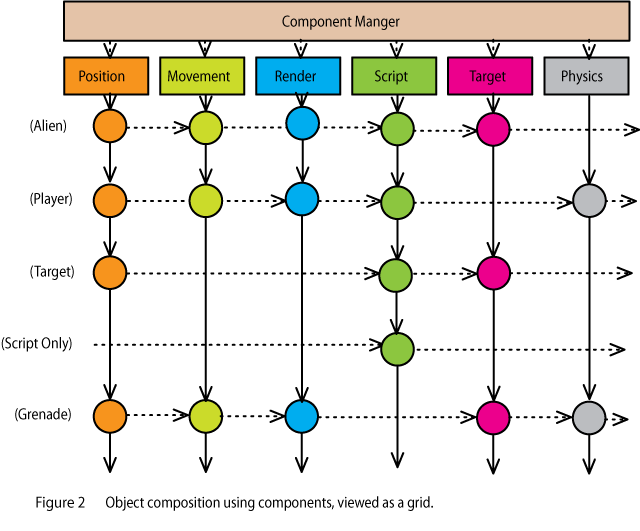
\includegraphics[width=\textwidth]{Fig-2.png}
\caption{Component Diagram}
\label{fig:comp}
\end{figure}

\subsection*{Simulator}
The core of the simulator is a basic ecological simulation. This N-body simulation will track organisms and systems within the world and apply various rules of growth, mutation, and predation upon entities. The simulator will expose the current location of each simulated object at regular intervals as a list of 2D cartesian coordinates and list of characteristics. This stream will be output to the screen or sent to a web browser which will interpret/display the results in a graphical manner, likely a 2D plot of pixels representing organisms.

\subsection*{Visualization}
Visualization is a core component of the project deliverable. However we have not decided to use a local 2D output or to output the data graphically through a web browser (possibly over WebGL).